%************************************************
\chapter[Glycolonitrile Chemistry]{Case study: Glycolonitrile Chemistry}
\label{ch:casestudy2} %
%************************************************

\definecolor{mygray}{gray}{0.9}
\definecolor{myBlue}{rgb}{0.0, 0.2, 0.6}
\definecolor{myGreen}{rgb}{0.1, 0.5, 0.0}
\definecolor{myBrown}{rgb} {0.43, 0.21, 0.1}
\definecolor{myCyan}{rgb}{0.0, 0.58, 0.71}
\definecolor{myBlue2}{rgb}{0.36, 0.57, 0.9}
\definecolor{myRed}{rgb}{0.87, 0.36, 0.51}

{\sffamily\slshape The text in this chapter is identical to Section 4 of the published version of the preprint at \href{https://arxiv.org/abs/2504.10609}{arXiv:2504.10609}.\\}

In this chapter, we apply the methods from Chapter~\ref{ch:refined_model} to a reaction network generated in silico from glycolonitrile (or more formally 2-hydroxyethanenitrile), ammonia (NH$_3$), and water (H$_2$O), a network previously studied in \cite{implemented_CRN}. The choice of 2-hydroxyethanenitrile as the starting molecule was driven by the fact that it has been reported to occur in interstellar medium as a product of the condensation of methanal with hydrogen cyanide and act as a precursor to important molecules in pre-biotic systems~\cite{MeCN_precursor}. The previous work~\cite{implemented_CRN} constructed a free-energy map of the molecules that might be present when 2-hydroxyethanenitrile reacts with water and ammonia using computationally-intensive density functional theory calculations. It focused on finding thermodynamic sinks and kinetic barriers in the different regions of the free energy landscape.

\section{Network Generation}

In this chapter, the network was expanded using the graph transformation based generative framework M{\O}D \cite{mod_web}. The generation of the network, starting from the three above-mentioned molecules was done through the recursive application of the three graph transformation rules shown in Figure~\ref{fig:graphTransformationRules}.
A graph transformation rules (to repeat what was already stated in Chapter~\ref{ch:casestudy1}) is a template representing a class of reactions, which share the same set of atoms involved in the reaction, with similar changes in the bond set. The left hand side of the rules is a subgraph (representing a molecular fragment), which can be rewritten as the subgraph on the right hand side, when a match is found in one of the graphs representing molecules already present in the reaction network. This executes a reaction, adding the new product molecules and the reaction the reaction network, and expands the molecular space.

\begin{figure}[!t]
    \centering
    \begin{subfigure}{\textwidth}
        \centering
        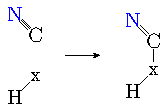
\includegraphics[scale=1.5]{graphics/chapter5/rule0.pdf}
        \caption{Addition to a cyanide: in this rule \texttt{x} $\in$ \{N, O\}, representing the addition of an amide nitrogen or hydroxyl oxygen to the nitrile bond respectively.}
        \label{fig: rule0}
    \end{subfigure}
    \\
    \vspace{0.5cm}
    \begin{subfigure}{\textwidth}
        \centering
        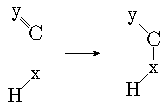
\includegraphics[scale=1.5]{graphics/chapter5/rule1.pdf}
        \caption{Addition to an imine or carbonyl: in this rule \texttt{x}, \texttt{y} $\in$ \{N, O\}, representing the addition of an amide nitrogen or hydroxyl oxygen to an amide or hydroxyl bond respectively. This single rule encapsulates $2^2 = 4$ individual rules depending on the instantiation of \texttt{x} and \texttt{y}.}
        \label{fig: rule1}
    \end{subfigure}
    \\
    \vspace{0.5cm}
    \begin{subfigure}{\textwidth}
        \centering
        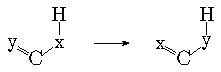
\includegraphics[scale=1.5]{graphics/chapter5/rule2.pdf}
        \caption{1,3 hydrogen shift: in this rule \texttt{x}, \texttt{y} $\in$ \{C, N, O\}, representing the shift of a double bond as in tautomerism. When \texttt{x}$\equiv$O and \texttt{y}$\equiv$O it is keto-enol tautomerism, \texttt{x}$\equiv$N and \texttt{y}$\equiv$N is imine-enamine tautomerism, \texttt{x}$\equiv$N and \texttt{y}$\equiv$O is amine-iminol tautomerism and \texttt{x}$\equiv$C and \texttt{y}$\equiv$C is an allylic shift of the double bond. This single rule encapsulates $3\times 3 = 9$ individual rules depending on the instantiation of \texttt{x} and \texttt{y}.}
        \label{fig: rule2}
    \end{subfigure}
    \vspace{0.2cm}
    \caption{The graph transformation rules used to expand the molecular space and generate the network. The inverse of all the three graph transofrmation rules were also used while generating the reaction network.}
    \label{fig:graphTransformationRules}
\end{figure}

\begin{figure}[!t]
	\centering
	\vspace{0.5cm}
    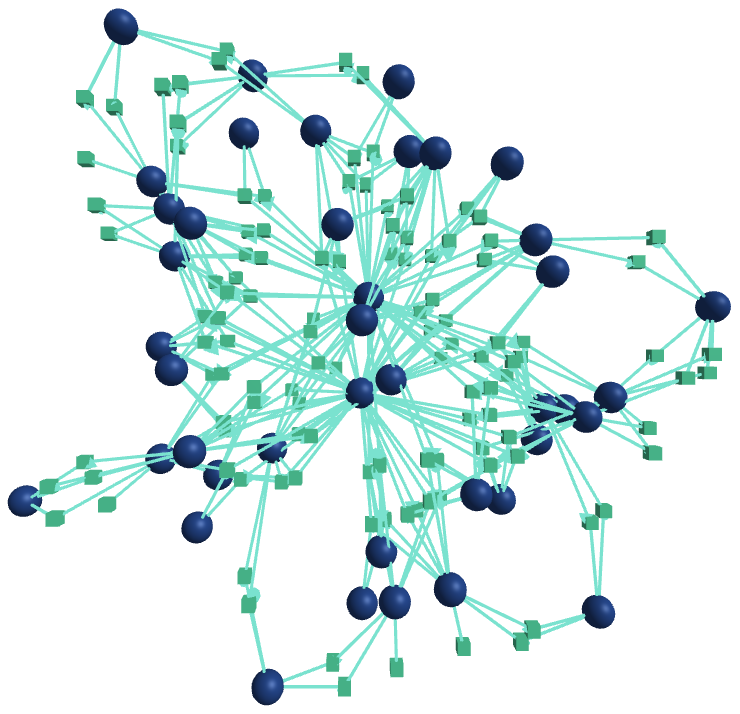
\includegraphics[width=0.8\textwidth]{graphics/chapter5/reactionNetworkChapter5.png}
    \vspace{0.5cm}
    \caption{An abstract representation of the generated reaction network with $44$ vertices (blue circles) and $116$ hyperedges (green squares), on which the working of the method proposed in Chapter~\ref{ch:refined_model} was demonstrated.}
    \label{fig: hypergraphRNChapter5}
\end{figure}

Molecules with up to two carbon, four nitrogen, and four oxygen atoms were included in the generated network for comparability with \cite{implemented_CRN}, which considered molecules with two carbon atoms only. The constructed reaction network had $44$ vertices and $116$ hyperedges, and shown in Figure~\ref{fig: hypergraphRNChapter5}. 
A list of molecules and reactions in the generated network is available in the GitHub data repository.  
To find probable pathways to biologically important molecules of glycine and glycolic acid, the structures of which are shown in Figure~\ref{fig:target0} and~\ref{fig:target1} respectively, using glycolonitrile, NH$_3$, and H$_2$O, an ILP was formulated to query the desired pathways.
The formulated ILP had $336$ variables and $1561$ constraints.
The reason for choosing glycine is that it is the simplest amino acid and can be considered as the building block of proteins which are essential for life. Glycolic acid is also widespread in nature in the form of glycolate salts which are produced during photorespiration in plants.
 
\begin{figure}[!t]
    \centering
    \begin{subfigure}{0.45\textwidth}
        \centering
        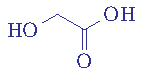
\includegraphics[scale=1.0]{graphics/chapter5/glycine.pdf}
        \caption{glycine}
        \label{fig:target0}
    \end{subfigure}
    \hfill
    \begin{subfigure}{0.45\textwidth}
        \centering
        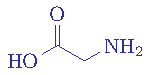
\includegraphics[scale=1.0]{graphics/chapter5/glycolic acid.pdf}
        \caption{glycolic acid}
        \label{fig:target1}
    \end{subfigure}
    \caption{target molecules in the flow query.}
    \label{fig:targetMolecules}
\end{figure}

\section{Pathways to Glycine}

The five best scoring pathways to the target glycine is depicted in Figure \ref{fig:pathway1}.
The structures for the molecules in the corresponding vertices is listed in Table \ref{tab:molecular_structures1} and the weights assigned to the hyperedges listed in Table \ref{tab:pathways1}.
The \textcolor{myBlue}{best scoring pathway} scores $143118$ on the chosen objective \eqref{proposed_objective} and proceeds through 2-iminoethanal ($v_6$), a pre-biotic intermediate hypothesized to be of significance. 
A water molecule acts as a catalyst in this pathway since it is used in reaction $e_1$ and generated back in reaction $e_4$. 
The \textcolor{myGreen}{second best pathway} scores $143190$ on the objective \eqref{proposed_objective}. The last two reactions are the same for both (in fact, for all \emph{five}) pathways. 
This second best pathway uses an ammonia molecule as a catalyst, molecules with a higher chemical potential (under unit concentrations) and reactions with higher energy barriers. The sum of the energy barriers for the reactions in this pathway is $200.02$ kJ mol$^{-1}$ as opposed to $128.74$ kJ mol$^{-1}$ for the best pathway. 
One might note that the difference in the objective value of the best and the second-best solutions, that is $143190-143118 = 72$ is entirely due to the difference in the sum of the energy barriers of the reactions along the pathway ($(200 - 128)$ kJ mol$^{-1} = 72$ kJ mol$^{-1}$) or the first part of the ovjective \eqref{proposed_objective} because both the pathways have the same length. Both pathways consist of $6$ reactions and the second part of the objective \eqref{proposed_objective} is the same for both solutions.

The \textcolor{myBrown}{third pathway} branches off the second pathway and merges into the first, with a different reaction $e_4$ eliminating an ammonia molecule. This ammonia molecules was added to glycolonitrile in the first step and therefore, acts as a catalyst in the pathway.
The \textcolor{myCyan}{fourth pathway} uses a different molecule instead of iminoacetaldehyde, which has a higher chemical potential, hence is ranked lower than the previous three. 
The \textcolor{myBlue2}{fifth pathway} has \emph{eight} reactions, while the previous four had seven reactions. Despite having a lower sum of the energy barriers ($152.90$ kJ mol$^{-1}$), it is ranked lower than the previous three pathways because it is longer.
This exemplifies how the length of the pathways affects its ranking through the second part of the objective \eqref{proposed_objective}.
Figure \ref{fig:pathway1} shows how interconnected the individual different pathways in the network might be, often with parallel branches and cross-connections, which leads to complex behavior of the system. 

The estimated energy barriers for the reactions used in the reported pathways in Figure \ref{fig:pathway1} is presented in Table \ref{tab:pathways1}. Table \ref{tab:pathways1} consists of five columns that list the assigned weights for the hyperedges in the pathways shown in Figure \ref{fig:pathway1}. 
The shaded cells indicate hyperedges that have already been used in a previously enumerated pathway. For instance, all five pathways in Figure \ref{fig:pathway1} share the final two reactions. Consequently, the next four pathways reuse the last two reactions of the first pathway, and the last two rows for the corresponding columns are shaded to reflect this overlap.  

Ab initio molecular dynamics has been used in a previous work~\cite{crn_expand_qm3,glycine_pathway} to simulate the Urey-Miller experiment and find possible pathways to glycine in a prebiotic setting. The reported pathways in~\cite{crn_expand_qm3} also contain reactions catalysed by water and ammonia. The reported pathways to glycine in~\cite{crn_expand_qm3} proceeds through a singlet carbene intermediate, while those in~\cite{glycine_pathway} has a molecule with a three-membered ring, oxiranimine, as an intermediate. However, in the current work, there were no reaction templates used which might lead to the formation of a carbene-like molecule or a three-cycle in a molecule in the generated network. Hence, such a pathway was not observed. Carbenes and three-cycles are highly reactive intermediates, and their formation is a high energy process. On the whole, the pathways presented in this work have much lower reported energy barriers than that reported in these two studies.


\begin{figure}[!thb]
    \centering
    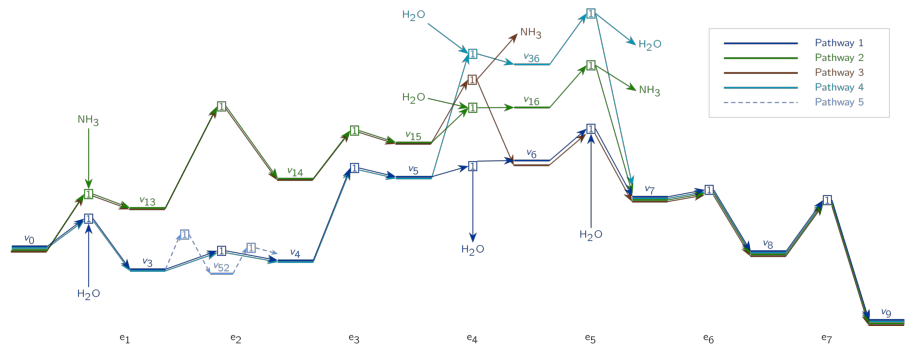
\includegraphics[width=\linewidth]{graphics/chapter5/pathway1.pdf}
    \vspace{0.4cm}\\
    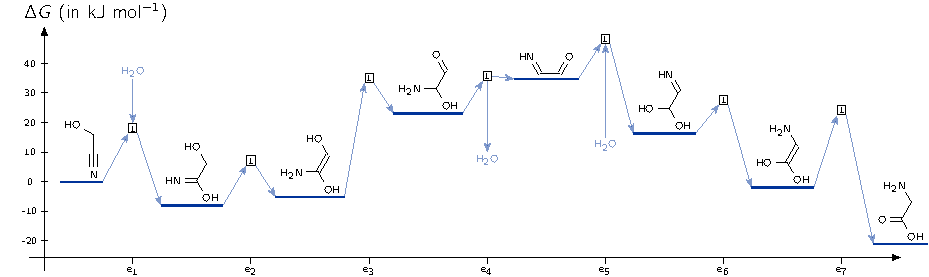
\includegraphics[width=\linewidth]{graphics/chapter5/bestPathway1.pdf}
    \vspace{0.1cm}
    \caption{Top: A schematic depiction of the five best pathways to glycine according to the chosen scoring function (energy levels not shown exactly to scale).   
    Bottom: The energy profile of the best-scoring pathway (in blue) from above (energy levels shown to scale) wth the molecular structures explicitly shown.}
    \label{fig:pathway1}
\end{figure}

\begin{figure}[!thb]
	\vspace{0.5cm}
	\begin{subfigure}{0.65\textwidth}
    	\centering
    	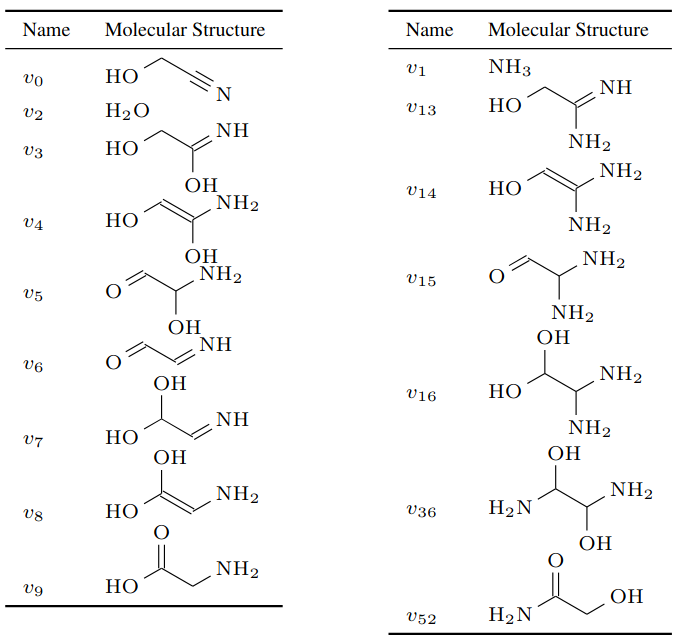
\includegraphics[scale=0.3]{graphics/chapter5/molStrucPathway1.png}
    	\caption{Molecular graphs in the pathways in Figure \ref{fig:pathway1}.}
    	\label{tab:molecular_structures1}
    \end{subfigure}%
    \begin{subfigure}{0.3\textwidth}
    	\centering
    	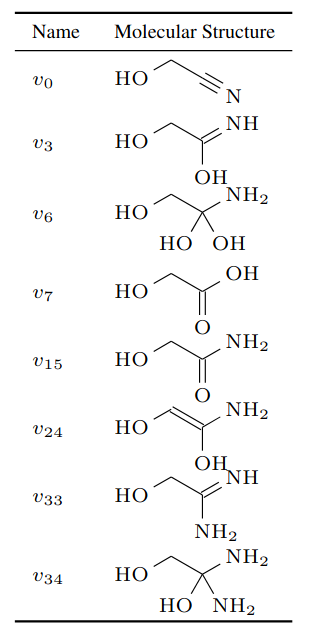
\includegraphics[scale=0.3]{graphics/chapter5/molStrucPathway2.png}
    	\caption{and in Figure \ref{fig:pathway2}}
    	\label{tab:molecular_structures2}
    \end{subfigure}
    \caption{List of the molecular structures corresponding to the the labeled vertices in the pathways in Figures~\ref{fig:pathway1} and~\ref{fig:pathway2}.}
\end{figure}

\begin{table}[!h]
    \centering
    \vspace{1cm}
    \begin{footnotesize}
    \begin{adjustbox}{angle=90}
    \begin{tabular}{lrrrrr}
        \toprule
        Reaction\hspace{0.2cm} & \multicolumn{5}{c}{Energy barriers (in kJ mol$^{-1}$)} \\
        count & \hspace{1cm}\textcolor{myBlue}{pathway 1} & \hspace{1cm}\textcolor{myGreen}{pathway 2} & \hspace{1cm}\textcolor{myBrown}{pathway 3} & \hspace{1cm}\textcolor{myCyan}{pathway 4} & \hspace{1cm}\textcolor{myBlue2}{pathway 5} \\
        \midrule
        \multirow{2}{*}{$e_1$} & $13.95$ & $33.18$ & \cellcolor{mygray}$33.18$ & \cellcolor{mygray}$13.95$ & \cellcolor{mygray}$13.95$\\
        & $(v_0+v_2, v_3)$ & $(v_0+v_1, v_{13})$ & \cellcolor{mygray}$(v_0+v_1, v_{13})$ & \cellcolor{mygray}$(v_0+v_2, v_3)$ & \cellcolor{mygray}$(v_0+v_2, v_3)$  \\
        \multirow{2}{*}{$e_2$} & $7.67$ & $64.17$ & \cellcolor{mygray}$64.17$ & \cellcolor{mygray}$7.67$ & $18.67, 13.15$\\
        & $(v_3, v_4)$ & $(v_{13}, v_{14})$ & \cellcolor{mygray}$(v_{13}, v_{14})$ & \cellcolor{mygray}$(v_3, v_4)$ & $(v_3, v_{52}, v_4)$ \\
        \multirow{2}{*}{$e_3$} & $57.69$ & $28.40$ & \cellcolor{mygray}$28.40$ & \cellcolor{mygray}$57.69$ & \cellcolor{mygray}$57.69$\\
        & $(v_4, v_5)$ & $(v_{14}, v_{15})$ & \cellcolor{mygray}$(v_{14}, v_{15})$ & \cellcolor{mygray}$(v_4, v_5)$ & \cellcolor{mygray}$(v_4, v_5)$\\
        \multirow{2}{*}{$e_4$} & $1.67$ & $19.86$ & $29.35$ & $67.36$ & \cellcolor{mygray}$1.67$\\
        & $(v_5, v_6+v_2)$ & $(v_{15}+v_2, v_{16})$ & $(v_{15}, v_6+v_1)$ & $(v_5+v_2, v_{36})$ & \cellcolor{mygray}$(v_5, v_6+v_2)$\\
        \multirow{2}{*}{$e_5$} & $17.14$ & $23.79$ & \cellcolor{mygray}$17.14$ & $60.84$ & \cellcolor{mygray}$17.14$ \\\
        & $(v_6+v_2, v_7)$ & $(v_{16}, v_7+v_1)$ & \cellcolor{mygray}$(v_6+v_2, v_7)$& $(v_{36}, v_7+v_2)$ & \cellcolor{mygray}$(v_6+v_2, v_7)$\\
        \multirow{2}{*}{$e_6$} & $0.19$ & \cellcolor{mygray}$0.19$ & \cellcolor{mygray}$0.19$ & \cellcolor{mygray}$0.19$ & \cellcolor{mygray}$0.19$ \\
        & $(v_7, v_8)$ & \cellcolor{mygray}$(v_7, v_8)$ & \cellcolor{mygray}$(v_7, v_8)$ & \cellcolor{mygray}$(v_7, v_8)$ & \cellcolor{mygray}$(v_7, v_8)$\\
        \multirow{2}{*}{$e_7$} & $30.42$ & \cellcolor{mygray}$30.42$ & \cellcolor{mygray}$30.42$ & \cellcolor{mygray}$30.42$ & \cellcolor{mygray}$30.42$ \\
        & $(v_8, v_9)$ & \cellcolor{mygray}$(v_8, v_9)$ & \cellcolor{mygray}$(v_8, v_9)$ & \cellcolor{mygray}$(v_8, v_9)$ & \cellcolor{mygray}$(v_8, v_9)$\\
        \midrule
        sum & $128.74$ & $200.02$ & $202.85$ & $238.13$ & $152.90$ \\
        \bottomrule
    \end{tabular}
    \end{adjustbox}
    \end{footnotesize}
    \vspace{1cm}
    \caption{From the left, the columns list the weights assigned to the hyperedges along with the sum of the weights, for the five pathways in Figure \ref{fig:pathway1}.}
    \label{tab:pathways1}
\end{table}

\begin{table}[!h]
    \centering
    \vspace{0.5cm}
    \begin{footnotesize}
    \begin{adjustbox}{angle=90}
    \begin{tabular}{lrrrrrr}
        \toprule
        Reaction\hspace{0.2cm} & \multicolumn{6}{c}{Energy barrier} \\
        count & \hspace{0.5cm}\textcolor{myBlue}{pathway 1} & \hspace{0.5cm}\textcolor{myGreen}{pathway 2} & \hspace{0.5cm}\textcolor{myBrown}{pathway 3} & \hspace{0.5cm}\textcolor{myCyan}{pathway 4} & \hspace{0.5cm}\textcolor{myBlue2}{pathway 5} & \hspace{0.5cm}\textcolor{myRed}{pathway 6} \\
        \midrule
        \multirow{2}{*}{$e_1$} & $13.95$ & \cellcolor{mygray}$13.95$ & \cellcolor{mygray}$13.95$ & \cellcolor{mygray}$33.18$ & \cellcolor{mygray}$13.95$ & \cellcolor{mygray}$33.18$\\
        & $(v_0+v_2,v_3)$ & \cellcolor{mygray}$(v_0+v_2,v_3)$ & \cellcolor{mygray}$(v_0+v_2,v_3)$ & \cellcolor{mygray}$(v_0+v_1,v_{33})$ & \cellcolor{mygray}$(v_0+v_2,v_3)$ & \cellcolor{mygray}$(v_0+v_1,v_{3}3)$\\
        \multirow{2}{*}{$e_2$} & & & $7.67$ & $48.612$ & $80.53$ & \cellcolor{mygray}$48.61$\\
        & & & $(v_3, v_{24})$ & $(v_{33}+v_2, v_{34})$ & $(v_3+v_1, v_{34})$ & \cellcolor{mygray}$(v_{33}+v_2, v_{34})$\\
        \multirow{2}{*}{$e_3$} & $26.61$ & $18.68$ & $11.76$ & $43.64$ & \cellcolor{mygray}$43.64$ & $33.08$\\
        & $(v_3+v_2, v_6)$ & $(v_3, v_{15})$ & $(v_{24}, v_{15})$ & $(v_{34}, v_{15}+v_1)$ & \cellcolor{mygray}$(v_{34}, v_{15}+v_1)$ & $(v_{34}, v_3+v_1)$\\
        \multirow{2}{*}{$e_4$} & & $0.62$ & \cellcolor{mygray}$0.62$ & \cellcolor{mygray}$0.62$ & \cellcolor{mygray}$0.62$ & \cellcolor{mygray}$0.62$\\
        & & $(v_{15}+v_2,v_6)$ & \cellcolor{mygray}$(v_{15}+v_2,v_6)$ & \cellcolor{mygray}$(v_{15}+v_2,v_6)$ & \cellcolor{mygray}$(v_{15}+v_2,v_6)$ & \cellcolor{mygray}$(v_3+v_2,v_6)$\\
        \multirow{2}{*}{$e_5$} & $74.62$ & \cellcolor{mygray}$74.62$ & \cellcolor{mygray}$74.62$ & \cellcolor{mygray}$74.62$ & \cellcolor{mygray}$74.62$ & \cellcolor{mygray}$74.62$ \\
        & $(v_6, v_7+v_1)$ & \cellcolor{mygray}$(v_6, v_7+v_1)$ & \cellcolor{mygray}$(v_6, v_7+v_1)$ & \cellcolor{mygray}$(v_6, v_7+v_1)$ & \cellcolor{mygray}$(v_6, v_7+v_1)$ & \cellcolor{mygray}$(v_6, v_7+v_1)$\\
        \midrule
        sum & $118.19$ & $107.87$ & $108.63$ & $200.68$ & $213.38$ & $219.11$  \\
        \bottomrule
    \end{tabular}
    \end{adjustbox}
    \end{footnotesize}
    \vspace{0.5cm}
    \caption{From the left, the columns list the weights assigned to the hyperedges along with the sum of the weights, for the six pathways in Figure \ref{fig:pathway2}.}
    \label{tab:pathways2}
\end{table}

\section{Pathways to Glyoxlic acid}

\begin{figure}[!t]
    \centering
    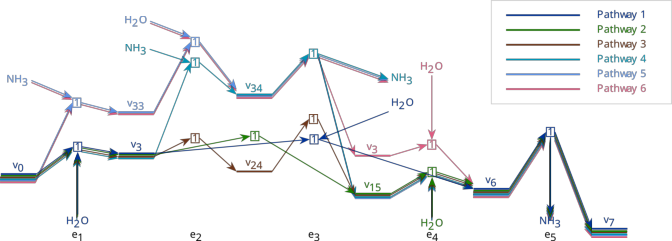
\includegraphics[width=\linewidth]{graphics/chapter5/pathway2.pdf}
    \caption{The six best pathways to glyoxlic acid according to the chosen scoring function.
    The best scoring pathway is depicted in blue, and the next best pathways in green, brown, cyan, azure and red. 
    The structures for the molecules for the vertices is listed in Table \ref{tab:molecular_structures2} and the weights assigned to the hyperedges listed in Table \ref{tab:pathways2}.}
    \label{fig:pathway2}
\end{figure}

\begin{figure}[!thb]
	\vspace{0.5cm}
    
\end{figure}

Another molecule of importance in prebiotic systems which appears in the generated network is 2-hydroxyethanoic acid, commonly known ad glycolic acid. During photorespiration plants produce glycolate. It can also be used as a monomer for various biodegradable polymers such as polyglycolic acid and poly(lactic-co-glycolic) acid. However, there have not been many studies on pathways to glyocolic acid from the precursor molecules in prebiotic systems.  
Figure \ref{fig:pathway2} shows the six best pathways to 2-hydroxyethanoic acid along with the molecules used in the pathway in Table~\ref{tab:molecular_structures2}. The \textcolor{myBlue}{best scoring pathway} has three reactions, the \textcolor{myGreen}{second best} has four reaction, while the rest involve five reactions. Despite the third-listed pathway having a lower sum of energy barriers ($108.63$ kJ mol$^{-1}$), it is ranked lower because it is longer, illustrating the effect of the second term in the objective \eqref{proposed_objective}. 

Table \ref{tab:pathways2} contains six columns that list the assigned weights for the hyperedges in the pathways illustrated in Figure \ref{fig:pathway2}. As in Table \ref{tab:pathways1}, the shaded cells indicate hyperedges that have already been used in a previously enumerated pathway. The specific hyperedge is mentioned below the energy barrier, with the reactants as the first element of the pair and the products as the second element. Individual molecules are separated by a `+', and the structures of the molecules the labels correspond to can be looked up from Table \ref{tab:molecular_structures2}. 

The expansion of the network shown in Figure~\ref{fig: hypergraphRNChapter5} took 67 seconds. It is quite faster than comparable methods using reaction templates without using graph transformation, molecular dynamics or potential energy search as done in~\cite{implemented_CRN}. Annotating the $116$ hyperedges with the energy barriers of the reactions as weights took around an hour. Using a neural network instead of more accurate traditional methods does lead to trade off of the accuracy for speed, but it allows scalability for larger networks. Formulating the ILP and enumerating the pathways in the network to the two target molecules using the objective function \eqref{proposed_objective} took around $52$ seconds. All the reported times are the average of $10$ runs on an AMD$^{\circledR}$ Ryzen 5 PRO 4650U CPU (2.1 GHz) utilizing $8$ threads.

